\documentclass[oneside,a4paper,spanish,links]{amca}
%
\usepackage{graphicx}
\usepackage{amsmath,amsfonts}
\usepackage[utf8]{inputenc}
\usepackage[spanish]{babel}

\title{MODELADO PARA LA RENDERIZACION FOTO-REALISTA DE PAN}

\author[a]{Rodrigo Baravalle}
\author[b]{Leonardo Scandolo}
\author[c]{Claudio Delrieux}
\author[d]{Cristian G. Bauza}
%
\affil[a]{Laboratorio de Sistemas Din\'amicos y Procesamiento de Se\~nales, FCEIA, Universidad Nacional de Rosario, CIFASIS-CONICET,
  Ocampo y Esmeralda, S2000EZP~Rosario, Argentina,
  baravalle@cifasis-conicet.gov.ar, \url{http://www.cifasis-conicet.gov.ar/grupo4.html}}
%
\affil[b]{Departamento de Ciencias de la Computaci\'on, FCEIA, Universidad Nacional de Rosario,
  Pellegrini 250, 2000~Rosario, Argentina,
  leonardo@fceia.unr.edu.ar, \url{http://web.fceia.unr.edu.ar/es/institucional/escuelas/118-departamento-ciencias-de-la-computacion-ecen.html}}

\affil[c]{Departamento de Ingenier\'ia El\'ectrica y de Computadoras, Universidad Nacional del Sur - IIIE-CONICET,
  Col\'on 80, 8000FTN~Bah\'ia Blanca, Argentina,
  cad@uns.edu.ar, \url{http://www.ingelec.uns.edu.ar/}}

\affil[d]{Instituto de Investigaci\'on PLADEMA- Facultad de Ciencias Exactas - Universidad Nacional del Centro, Campus Universitario,
  Paraje Arroyo Seco, (B7001BBO) Tandil, Buenos Aires, Argentina
  crgarcia@exa.unicen.edu.ar, \url{http://www.exa.unicen.edu.ar/es/d_investigacion/inst_pladema/index.html}}


%% NOTE: IF ALL AUTHORS BELONG TO THE SAME AFFILIATION
%% USE THE `\voidaffil' MACRO FOR THE AFFILIATION CODE.
%% Example:
%% \author[\voidaffil]{First A. Author}
%% \author[\voidaffil]{Second B. Author}
%% \author[\voidaffil]{Third C. Author}
%% \author[\voidaffil]{Fourth D. Author}
%% %
%% \affil[\voidaffil]{Grupo de Mec\'anica Computacional,
%% Universidad Nacional de Villa Carolina,
%% Los Alerces 3492, 4200 Villa Carolina, Argentina,
%% gmc@uncarolina.edu.ar, http://www.uncarolina.edu.ar/gmc}

\begin{document}
\vspace{3cm}

\maketitle

%% To set PDF METADATA: uncomment and replace fields in
%% UPPERCASE with appropriate values. 
%% 
%% \hypersetup{
%%   pdfauthor={AUTHORS},
%%   pdfkeywords={KEYWORDS},
%%   pdftitle={TITLE}
%% }
%%
%% For instance
%% \hypersetup{
%%   pdfauthor={Sponge B. and Star P.},
%%   pdfkeywords={multiphase flow, air-liquid mixtures},
%%   pdftitle={A new model for multi-phase flow}
%% }
%%
%% NOTE: To set the metadata is recommended but not absolutely
%% neccesary. 
%% This was done before with the \pdfinfo command,
%% but according to this post:
%% http://de.nntp2http.com/comp/text/tex/2008/12/5358fd061de9703a781885a5dcf98364.html
%% if `hyperref' is used, then you must use \hypersetup{} not \pdfinfo{}

\begin{keywords}
  Direct Volume Rendering, Pan, Tiempo Real.
\end{keywords}

\begin{abstract}
  El modelado foto-real\'istico de materiales con una estructura interna compleja presenta varios desaf\'ios en Computaci\'on Gr\'afica. Espec\'ificamente, la miga del pan es un material transl\'ucido cuya estructura es porosa, mostrando detalles en distintas escalas. Si se pretende obtener resultados foto-realistas, deben modelizarse fen\'omenos tales como sombras internas, oclusi\'on, transmitancia y absorci\'on. La soluci\'on t\'ipica en estos casos es la aplicaci\'on directa de la ecuaci\'on del rendering, es decir, utilizar iluminaci\'on global (ray tracing, path tracing). Sin embargo, estos m\'etodos presentan un costo computacional elevado y necesitan una malla 3D detallada del material.

El estado del arte en renderizaci\'on de materiales porosos utiliza un complejo procedimiento de captura donde la luz que es reflejada por el material es obtenida en distintos \'angulos. Esa informaci\'on es utilizada para reconstruir un modelo computacional del material. Si bien utilizando esta t\'ecnica es posible modelar alguna de las propiedades lum\'inicas deseadas, los costos computacionales asociados, el procedimiento de captura requerido y la baja variabilidad de la imagen resultante han provocado una dificultosa aplicaci\'on pr\'actica del m\'etodo.


En este trabajo proponemos el estudio e implementaci\'on en GPU de un modelo basado en {\em direct volume rendering} sobre un campo escalar representando la estructura de la miga de pan sin utilizar estructuras intermedias. Las im\'agenes obtenidas muestran resultados promisorios en tiempo real. La miga es representada a trav\'es de un campo escalar 3D, el cual es computado en dos pasos. El primero utiliza una generaci\'on a trav\'es de sistemas de part\'iculas, y el segundo aplica sistemas din\'amicos para evolucionar las part\'iculas, emulando el proceso de leudado y cocci\'on del pan.

\end{abstract}

\section{INTRODUCCION}

La apariencia de la miga de pan y otros materiales cocidos, como pizzas y budines, ha sido considerada un desaf\'io para renderizar debido a la compleja interacci\'on del material con la luz. Los costos computacionales asociados (almacenamiento de memoria y tiempo computacional) de estos procesos f\'isicos hacen que el renderizado sea impr\'actico en aquellas áreas donde la interactividad sea mandatoria. El crecimiento exponencial en poder de c\'omputo, provocado mayormente por el dise\~no masivamente paralelo de las placas gr\'aficas \citep{Yeo09,Harris06}, ha hecho posible simular algunos fen\'omenos de la luz mencionados en tiempos computacionales aceptables, sin embargo el campo es a\'un objeto de estudio \citep{Voglsam2013}.

Estos materiales poseen una geometr\'ia observable la cual representa de por s\'i un desaf\'io adicional. Estas estructuras porosas son el resultado de mecanismos complejos que involucran deformaciones f\'isicas y reacciones qu\'imicas. La producci\'on de pan presenta dos etapas: leudado y cocci\'on. Durante el leudado, la levadura genera $CO_{2}$, produciendo burbujas en la masa \citep{Shah1998}. El proceso de cocci\'on \citep{Mondal2008} modifica estas burbujas de distintas maneras \citep{Scanlon2001}, d\'andole al pan su estructura final. Se han hecho intentos de s\'intesis de esta estructura \citep{Cho2007}, pero el resultado es en realidad un proceso art\'istico. En este trabajo proponemos la utilizaci\'on de sistemas din\'amicos \citep{Strogatz2001} aplicados a la evoluci\'on de sistemas de part\'iculas \citep{Reeves83}, utilizando un trabajo que los autores realizaron previamente \citep{Baravalle2011}. Estos esfuerzos son un intento de imitar el leudado y la cocci\'on mencionados. Los sistemas de ecuaciones diferenciales describen adecuadamente el comportamiento de procesos muy complejos, como el clima, la dinámica de fluídos \citep{Stam1999}, etc. Esta idea se utiliza en este trabajo para modelar el crecimiento de burbujas en el interior de panes. Este proceso arroja como resultado una estrucura similar a burbujas sobre un fluido, lo cual puede observarse en distintos panes. En otros trabajos se computa el valor de la textura en cada voxel del dominio \citep{Perlin1989}, por lo cual no se requiere memoria para alojar la textura 3D, sin embargo estos m\'etodos requieren un enfoque estad\'istico que resulta inadecuado para capturar la distribuci\'on de las burbujas.

La estructura de datos utilizada en la representaci\'on de estas geometr\'ias influye fuertemente el renderizado de las mismas. Si se utiliza una malla tradicional 3D, la misma debe computarse a partir de un campo escalar previamente construido, utilizando t\'ecnicas como 
{\em marching cubes} \citep{Lorensen1987}. Este proceso podr\'ia no resultar trivial debido a la estructura porosa del material. Representar la miga de pan como una superficie resulta tambi\'en inadecuado, ya que existen estructuras (burbujas) sobre la misma, por lo cual soluciones t\'ipicas como utilizar funciones bidireccionales de distribuci\'on de reflectancia (BRDF) \citep{Kurt2009} no son factibles. Si bien existe una propuesta \citep{Tong2005}, ésta es demasiado compleja en su implementación, junto a un difícil proceso de captura asociado, la baja variabilidad en las im\'agenes resultantes y los costos computacionales del m\'etodo, han hecho que el mismo no sea utilizado de manera masiva. 

En este trabajo se propone la aplicaci\'on de Direct Volume Rendering (DVR) \citep{Levoy1988, Kratz2006} sobre un campo escalar para renderizar el interior de distintos objetos sometidos a un proceso de cocción. El método de DVR consiste en lanzar rayos desde una c\'amara virtual hacia el campo escalar, acumulando distintas propiedades para cada pixel. El m\'etodo no utiliza estructuras intermedias, simplificando el proceso de modelado. La forma exterior del material puede ser definida en tiempo real en la GPU, haciendo posible realizar cortes y deformaciones a la miga original. Adem\'as, la corteza del mismo se establece utilizando funciones de transferencia (definici\'on de distintas regiones en el espacio). Los resultados obtenidos son satisfactorios y se computan en tiempo real.

\section{MATERIALES Y METODOS}

\subsection{Sistemas de Part\'iculas}

Los primeros trabajos en computaci\'on gr\'afica utilizaron la geometr\'ia Euclideana para describir figuras. Es decir, combinando puntos, rectas, planos y otras primitivas. Si bien esta metodolog\'ia es \'util para representar construcciones matem\'aticas simples, la misma presenta dificultades sobre todo en el modelado de objetos naturales. Estas limitaciones pueden ser superadas en muchos casos utilizando geometría fractal \citep{Mandelbrot83}.

Distintas t\'ecnicas hicieron su aparici\'on para superar estos problemas. Los sistemas de part\'iculas \citep{Reeves83} suplieron la necesidad de trabajar con todo aquello que no tuviese superficie bien definida, como agua, fuego y humo \citep{Cords2008, Paiva2009,Muller2003}. Estos sistemas est\'an compuestos por entidades denominadas {\em part\'iculas}, las cuales modifican sus propiedades en el tiempo. Por ejemplo, se puede obtener una animaci\'on de fuegos artificiales definiendo un origen com\'un en el espacio para todas las part\'iculas, cambiando su posici\'on en el tiempo siguiendo par\'abolas levemente diferentes para cada una de ellas. Otras propiedades como el color y el tama\~no permiten definir fuego y humo. Las part\'iculas pueden tambi\'en afectarse mutuamente.

En un trabajo previo, \citep{Baravalle2011}, se emplearon distintos sistemas de part\'iculas en la s\'intesis de texturas. Cada part\'icula tomaba una posici\'on aleatoria en una imagen, y evolucionaba tratando de evitar otras part\'iculas, compitiendo de esta forma por posiciones dentro de la misma. Se obtuvieron resultados adecuados para im\'agenes de madera y pinturas art\'isticas. Las funciones de crecimiento utilizadas fueron crecimiento vertical, aleatorio, horizontal, y diagonal. En este trabajo nos proponemos extender el dominio al espacio 3D, controlando el crecimiento de las part\'iculas por medio de un sistema de ecuaciones diferenciales, imitando el proceso de leudado y cocci\'on del pan. De esta forma se obtiene una textura 3D representando el material.


\subsubsection{Algoritmo de modelado}

El prop\'osito de este algoritmo es producir una geometr\'ia la cual se renderizar\'a posteriormente. Por lo tanto, en lugar de devolver el color de una posici\'on espec\'ifica, el algoritmo genera un campo escalar compuesto de $0$s y $1$s ($0$ si la posici\'on contiene aire, $1$ si la misma contiene masa). Esta representaci\'on resulta adecuada para ser renderizada utilizando DVR.

El sistema consta de un conjunto de part\'iculas $P$,

\begin{equation}
  P = \{p_{1}, ... , p_{n}\}, n  \in \mathbb{N},
\end{equation}

\noindent una grilla $L_{N\times N \times N}, N \in \mathbb{N} $ (inicialmente $L_{xyz}=1$) de masa y aire como fue descripto previamente, y otra grilla $L2_{N\times N \times N}$, (inicialmente $L2_{xyz}=-1$) de posiciones donde cada celda almacena un único entero que indica qu\'e part\'icula es due\~na de la misma ($i$ si el elemento de la grilla pertenece al contorno o interior de la part\'icula $i$).

Cada elemento en $P$ posee las siguientes propiedades:

\begin{equation}
  p_{i} = \{O_{i}, C_{i}\}, 1 \le i \le n,
\end{equation}

\noindent donde:

\begin{itemize}
\item $O_{i} = \{o_{1}, ... , o_{n_{i}}\}$: (Ocupadas) vector (conjunto) de posiciones ocupadas por la part\'icula en $L$.

\item $C_{i} = \{c_{1}, ... , c_{m_{i}}\}$: (Contorno) vector (conjunto) de posiciones representando el {\em contorno} de la part\'icula en $L$.
\end{itemize}

El vector $O$ representa las posiciones que ser\'an afectadas por la part\'icula, y el contorno $C$ se utiliza para asegurar que las part\'iculas se eviten entre s\'i.

El algoritmo se describe, simplificadamente, en el siguiente pseudo-codigo: 

\begin{verbatim}
// Inicialización
t  = 0       // tiempo - iteración
P  = []      // partículas
// Geometría (burbuja,masa)  - iniciada a 1 (masa)
L  = matriz(MxMxM,1)  
L2 = matriz(MxMxM,-1) // Dominio de cada partícula - iniciada a -1
Para i de 1 a Cantidad_Particulas
    // Cada partícula toma una posición aleatoria en L
    x = aleatorio()
    y = aleatorio()
    O[i] = [[x,y]]
    C[i] = []
    // Se agrega cada posicion del vecindario
    Para todo v en vecindario(x,y)
        C[i] = agregar(v,C[i])
    P = agregar([O[i],C[i]],P)

// Crecimiento
Para t de 0 a tiempo_max
    Para i de 1 a Cantidad_Particulas
        si vecindario(P[i]) == vacio, morir()
        // h: vector x,y,z
        Para h en C[i]
            // Si la posición pertence a otra partícula,
            // elegir otra posición
            eliminar(h,C[i])
            si L2[h] != -1 y L2[h] != i 
                continuar
            sino, 
                L[h] = 0 // masa -> aire
                agregar(h,O[i])
                agregar(vecindario(h),C[i])
                // Marcar posiciones en L2 como i
                setear(vecindario(h),L2,i)
                setear(h,L2,i)
                // turno de la particula i+1
                siguiente_particula()
    
        

\end{verbatim} 

Cuando $t = 0$, un conjunto de part\'iculas iniciales toman posiciones aleatorias en la grilla. La posici\'on elegida es la primera posici\'on ocupada en $O$, adem\'as, el vecindario de $O$ es agregado a $C$. Cada part\'icula evoluciona en un intento por extender sus posiciones ocupadas ($O$), marcando posiciones en $L$. Las posiciones se toman de $C$. Cuando una part\'icula ocupa una posici\'on, la misma se elimina de $C$ y se agrega a $O$. Luego el vecindario de esa posici\'on se agrega a $C$ (es decir las posiciones que rodean inmediatamente a la posici\'on tomada). Las grillas se actualizan de la siguiente manera: $L$ se setea a $0$ en la posici\'on y $L2$ se setea con el valor $i$ en las posiciones que se agregan a $C$. Las part\'iculas s\'olo pueden crecer si el valor encontrado en $L2$ no pertenece a otra part\'icula. El tama\~no del vecindario es un par\'ametro que define la distancia entre part\'iculas. Si el vector $C$ est\'a vac\'io, la part\'icula {\em muere} ya que no puede continuar creciendo.

El algoritmo puede ser terminado en cualquier $t$ deseado. El mismo puede finalizar su c\'omputo ante determinados eventos, por ejemplo, cuando todas las posiciones de $L2$ fueron tomadas por part\'iculas, ya que no pueden realizarse progresos.

Variando el par\'ametro de distancia entre part\'iculas se obtienen distintas estructuras (ver Fig.~\ref{fg:fig1}). Las im\'agenes muestran ejemplos 2D (para mayor claridad) de crecimiento aleatorio de part\'iculas. La regi\'on blanca en las im\'agenes representa la masa restante luego del proceso.


\begin{figure*}[htb!]
  \centerline{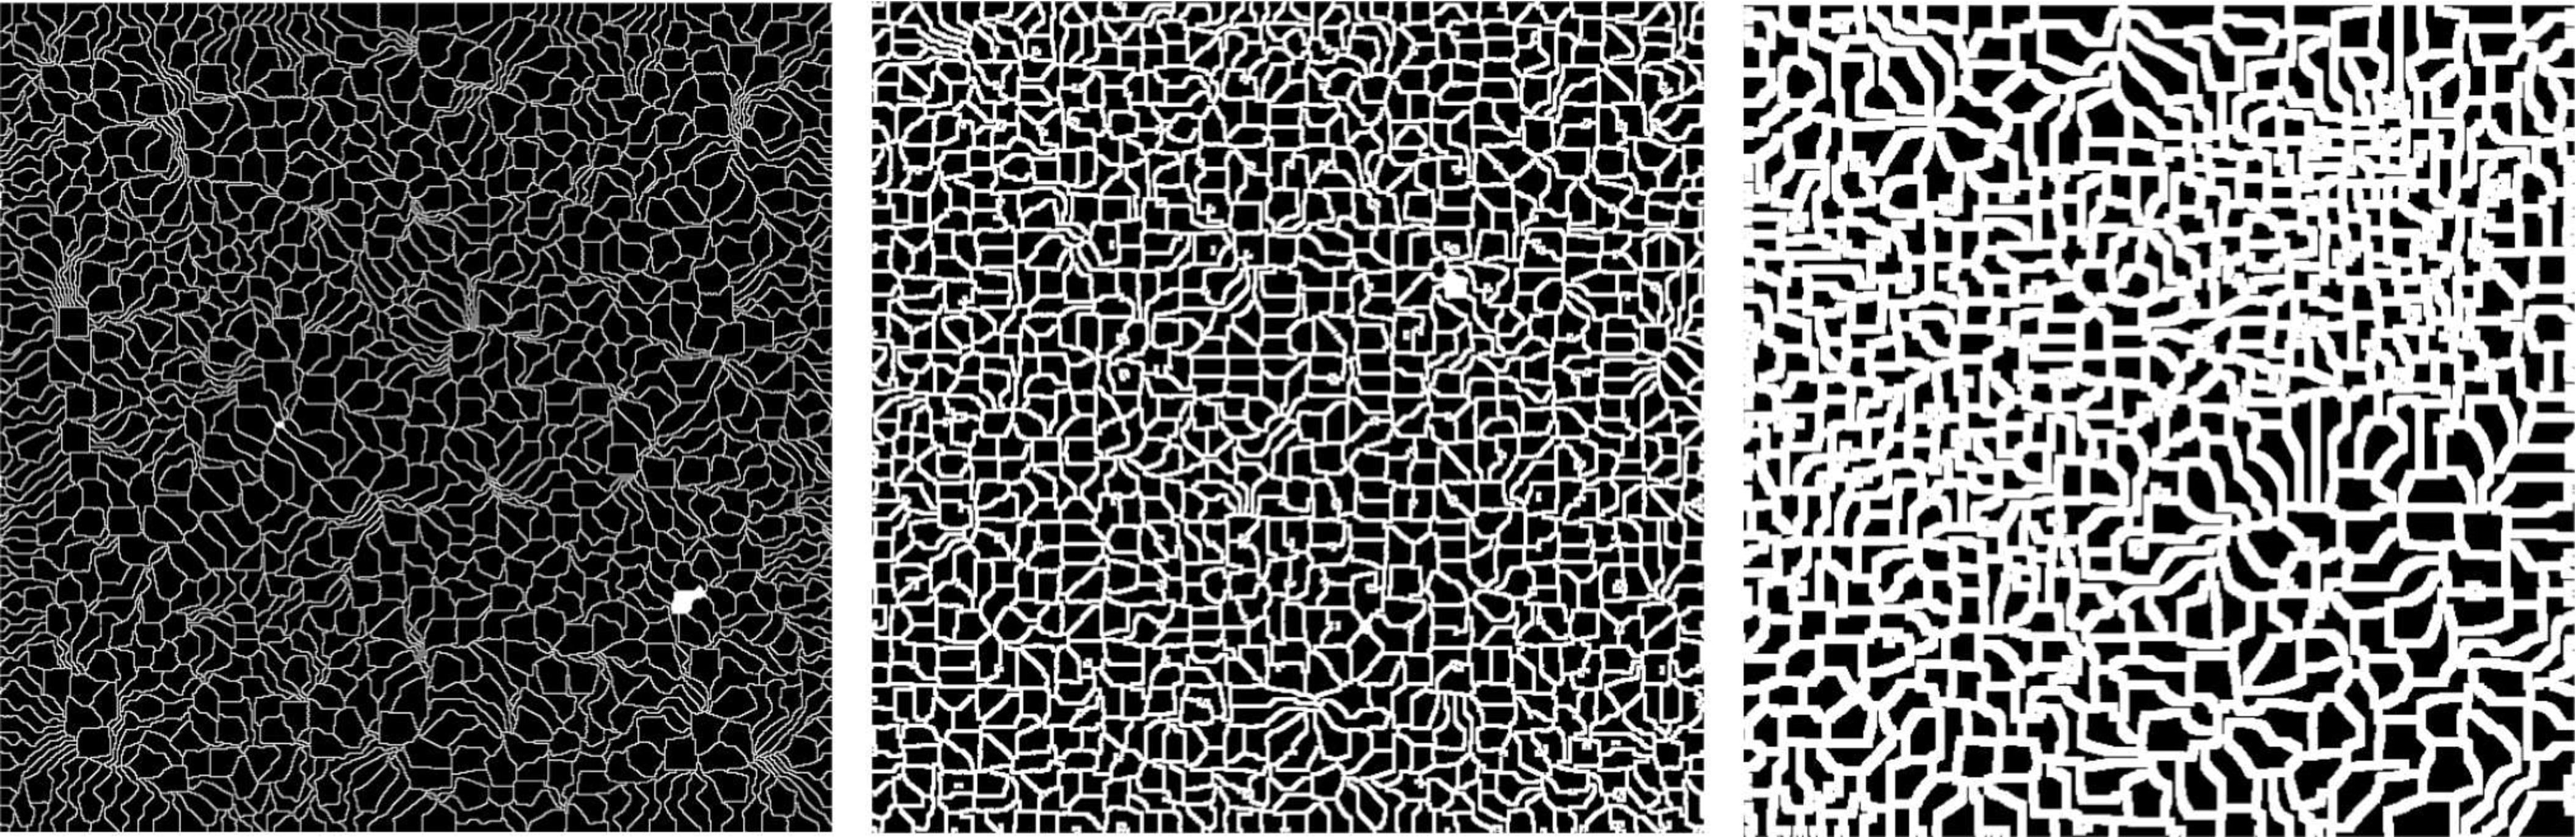
\includegraphics[scale=0.22]{fig1.pdf}}
  \caption{Diferentes separaciones entre part\'iculas utilizando el par\'ametro tama\~no del contorno. Izquierda: separaci\'on = 1, centro: separaci\'on = 2, derecha: separaci\'on = 4.}
  \label{fg:fig1}
\end{figure*}

Finalmente, el algoritmo devuelve la grilla $L$, la cual ser\'a renderizada posteriormente. En la siguiente secci\'on se explica la utilizaci\'on de sistemas din\'amicos en la evoluci\'on guiada de part\'iculas.

\subsection{Sistemas Din\'amicos}

La din\'amica es el estudio del {\em cambio}. Los estudios en din\'amica comenzaron hace ya va\-rios siglos con Isaac Newton. Las ecuaciones diferenciales son un resultado de sus estudios. Las mismas fueron dise\~nadas con el prop\'osito de tratar con la dificultad (o imposibilidad) de hallar soluciones anal\'iticas para determinados procesos din\'amicos. En primer lugar, se define un modelo matem\'atico del problema, del cual luego se obtienen 
las ecuaciones diferenciales asociadas. Se simula la evoluci\'on del sistema y se obtienen soluciones aproximadas en cada paso de la simulaci\'on. Estos sistemas tratan procesos que evolucionan con el tiempo, como la econom\'ia, la transferencia de calor, o el clima.

Los sistemas de ecuaciones diferenciales asociados se resuelven por medio de aproximaciones num\'ericas en cada instante de tiempo. El desarrollo de las computadoras en el \'ultimo siglo ha hecho posible que la disciplina se desarrolle en campos donde antes resultaba imposible, como por ejemplo Fractales \citep{Mandelbrot83} y Caos.

Los costos computacionales de estas soluciones dependen de la complejidad del problema y el n\'umero de ecuaciones del sistema. En este trabajo proponemos usar un sub-\'area de ecuaciones diferenciales, llamadas ecuaciones diferenciales ordinarias (ODE). En esta representaci\'on, el tiempo es tratado como la \'unica variable independiente.


De manera general, las ODEs se representan utilizando el siguiente sistema de ecuaciones:
\begin{equation} \label{eq:simple}  
  \begin{aligned}
    \dot{x_{1}} = f_{1}(x_{1},\ldots,x_{n}),\\
    \ldots\\
    \dot{x_{n}} = f_{n}(x_{1},\ldots,x_{n}),
  \end{aligned}
\end{equation}

\noindent donde $\dot{x_{i}}$ representa la derivada de $x_{i}$ con respecto
a $t$. Las variables $x_{i}$ y las funciones $f_{i}$ se definen de manera diferente para cada problema. En este caso, cada variable representa una coordenada cartesiana en el espacio, $x_{1}$ es $x$, $x_{2}$ es $y$ y $x_{3}$ es $z$. El conjunto de $f_{i}$ ser\'a definido tratando de capturar la estructura interna del pan. La siguiente secci\'on muestra como estos sistemas pueden describir la evoluci\'on de los sistemas de part\'iculas.

\subsection{Evoluci\'on de sistemas de part\'iculas utilizando sistemas din\'amicos}

La percepci\'on humana puede detectar patrones en la estructura de la miga de pan. Distintas observaciones pueden realizarse sobre la distribuci\'on de las burbujas en la misma (ver Fig.~\ref{fg:fig2}). Primero, la forma de las burbujas cercanas a la corteza tiende a estirarse paralelamente a la misma. Esto es resultado de la acci\'on de las elevadas temperaturas durante la cocci\'on de la masa. Tambi\'en resulta evidente que la estructura completa es similar a un fluido con la forma de la corteza.


\begin{figure*}[htb!]
  \centerline{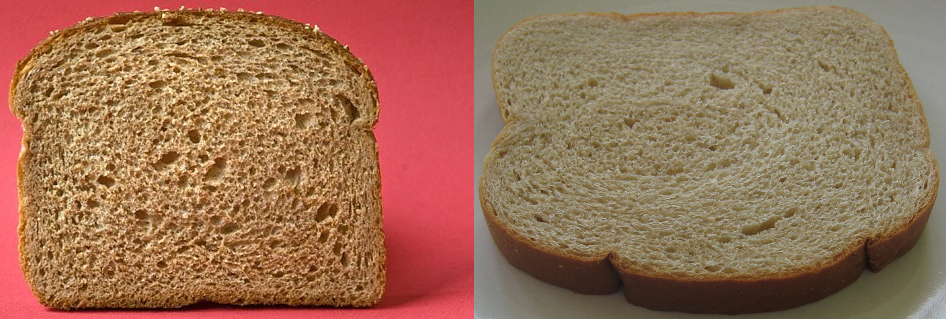
\includegraphics[scale=0.45]{fig2}}
  \caption{Im\'agenes de cortes reales de pan}
  \label{fg:fig2}
\end{figure*}

Por otro lado, los sistemas din\'amicos previamente presentados producen formas naturales (ver Fig.~\ref{fg:fig3}). En las im\'agenes pueden observarse c\'irculos y espirales, entre otras formas. Las im\'agenes se obtuvieron dibujando trayectorias sobre un plano, siguiendo distintas ODEs. Tres ODEs describen las din\'amicas presentes en las im\'agenes. A modo de ejemplo, la imagen de la izquierda es el resultado del siguiente conjunto de ecuaciones:

\begin{equation} \label{eq:simple}  
  \begin{aligned}
    \dot{x} &= x^{2}-y^{2}+1,\\
    \dot{y} &= 2xy+1.
  \end{aligned}
\end{equation}


\begin{figure*}[htb!]
  \centerline{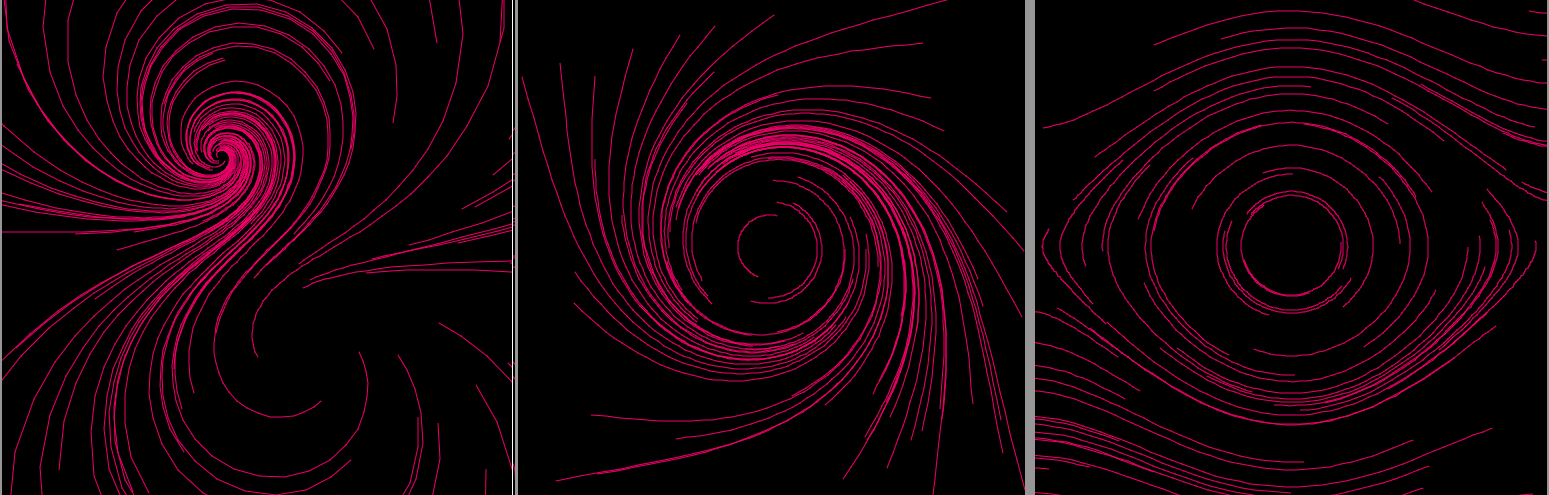
\includegraphics[scale=0.28]{fig3}}
  \caption{Sistemas din\'amicos en el plano.}
  \label{fg:fig3}
\end{figure*}

En los ejemplos se eligen posiciones aleatorias y luego el sistema se resuelve por medio de un {\em solver} Runge-Kutta de cuarto orden, el cual permite conocer la direcci\'on a tomar en cada punto por la trayectoria (en las im\'agenes se computaron trayectorias hacia adelante y hacia atrás en el tiempo para lograr una mejor visualizaci\'on). La imagen de la izquierda muestra un atractor y un repeledor claramente visibles. El centro de la espiral m\'as a la izquierda es un atractor (a medida que $t$ avanza, las trayectorias convergen hacia el punto), mientras que el otro centro es un repeledor. Los atractores pueden no ser puntuales, como muestran las restantes dos im\'agenes. La imagen de la derecha muestra atractores en forma de c\'irculos (las trayectorias ciclan por el c\'irculo).

Las part\'iculas producen distintos patrones al seguir las trayectorias definidas en el plano y el espacio. Esto se logra resolviendo num\'ericamete el sistema din\'amico en la posici\'on actual de la part\'icula, seleccionando como siguiente posici\'on de crecimiento aquella posici\'on del contorno que mejor aproxima la soluci\'on del sistema din\'amico. Las part\'iculas se deforman de forma global en un patr\'on que es visualmente similar a las trayectorias que produce el sistema (ver Fig.~\ref{fg:fig4}). En las im\'agenes, de izquierda a derecha se decrementa la {\em aleatoriedad} de las trayectorias. El par\'ametro aleatoriedad seteado a $0.1$ genera la imagen de la derecha, lo cual quiere decir que las burbujas siguen el sistema con una probabilidad de $0.9$. La probabilidad se define como $1-aleatoriedad$, donde $0 \leq aleatoriedad \leq 1$. Las ecuaciones del sistema son las mismas que las de la imagen derecha mostrada en Fig.~\ref{fg:fig3}. Estos patrones pueden ser utilizados adem\'as en otros materiales cocidos, variando el par\'ametro de aleatoriedad. Distintos sistemas de ecuaciones pueden utilizarse para definir distintos patrones.

\begin{figure*}[htb!]
  \centerline{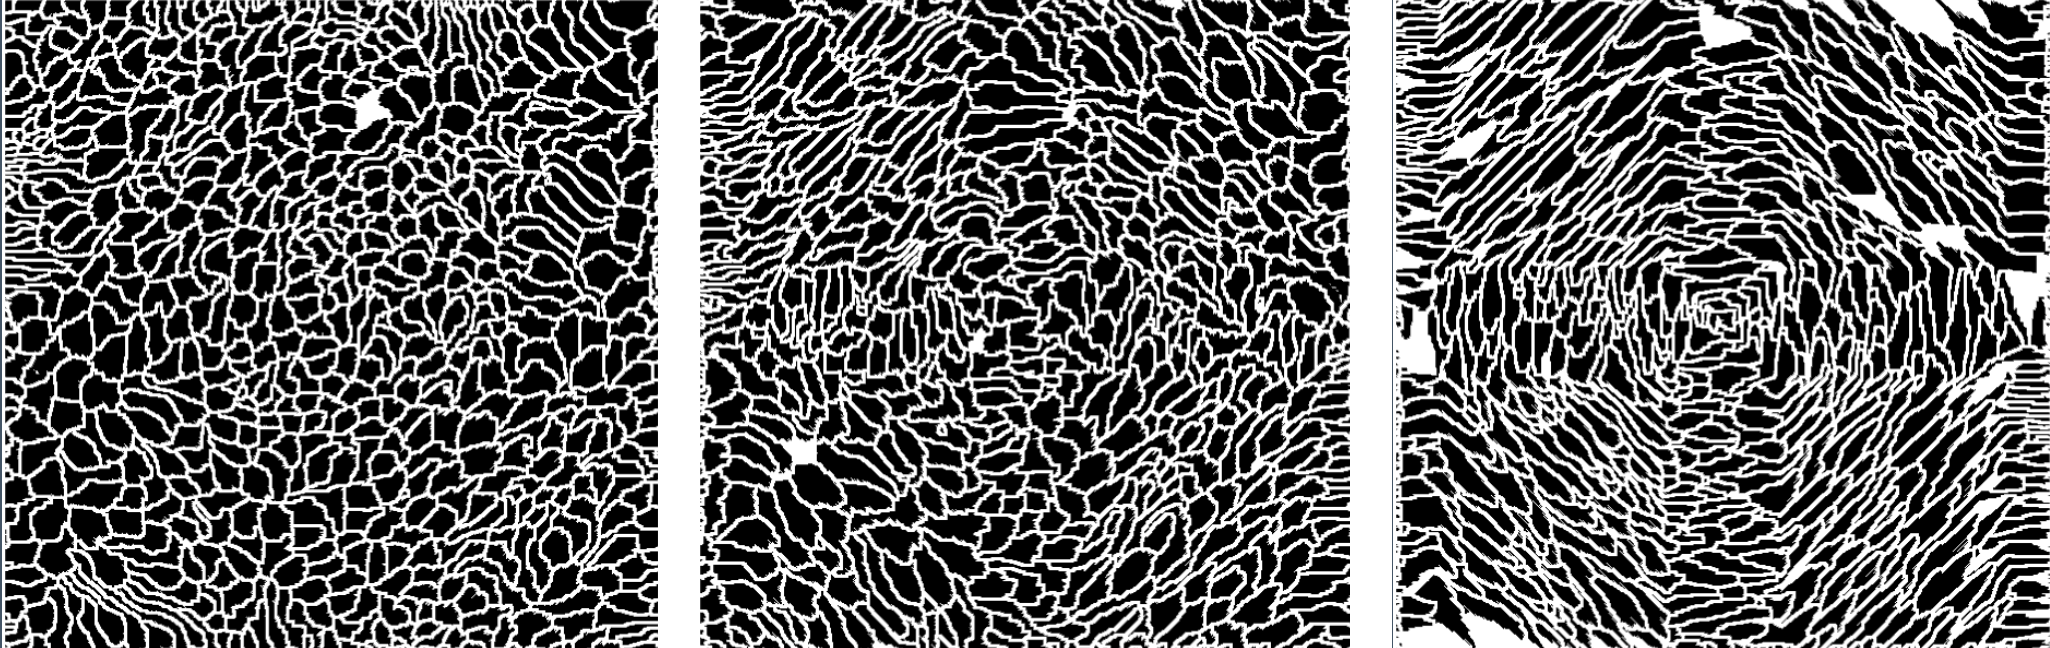
\includegraphics[scale=0.21]{fig4}}
  \caption{Sistemas din\'amicos aplicados en sistemas de part\'iculas. Efecto del pa\'ametro {\em aleatoriedad}. De izquierda a derecha, aleatoriedad: 0.3,0.2,0.1 respectivamente. }
  \label{fg:fig4}
\end{figure*}

La siguiente secci\'on muestra c\'omo estas particulas modificadas son renderizadas.

\subsection{Algoritmo de renderizado}

En esta sección explicaremos la teoría de la técnica de DVR y se
presentarán algunos aspectos de la implementación usada en este
trabajo.

\subsubsection{Direct volume rendering}

La técnica de DVR tiene como objetivo crear una representación
bidimensional de un vo\-lu\-men definido por una función de densidad
tridimensional. Para ello, se emiten rayos desde el punto de vista de
una camara en una escena virtual y se utiliza la función de densidad
para calcular la cantidad de luz que la cámara recibe en la dirección
del rayo. Para esto se evalúa la función de densidad en el camino del
rayo y se usan los valores adquiridos para aproximar el efecto de
varios fenómenos lumínicos, como pueden ser la extinción,
transmitancia, o dispersión lumínica, entre otros. La información
obtenida de procesar todos los rayos se usa para definir el color de
los pixeles en la imagen final.

La radiancia es la cantidad de luz que pasa, o es emitida, desde un
punto y atraviesa un determinado ángulo sólido. En el contexto de DVR,
el medio que los rayos atraviesan, y que es definido por una función
de densidad, es considerado como emisivo. Por lo tanto, cuando se
busca calcular la cantidad de luz recibida en la dirección de un rayo,
lo que se hace es aproximar la radiancia recibida de un punto distante
siguiendo la dirección del rayo. El valor de la radiancia es
aproximado como la suma de una radiancia de fondo y la radiancia
emitida por el medio por el cuál se mueve el rayo \citep{Kratz2006} :

\begin{equation} \label{eq:general_radiance}  
  L(p_n) = L_b + \int_{p_0}^{p_n} \frac{\partial L(t)}{\partial p} \, dt,
\end{equation}

\noindent donde $L_b$ es la radiancia de fondo, $p_0$ y $p_n$ son los
puntos inspeccionados en la dirección del rayo más cercano y más
lejano respectivamente, $L(t)$ es la radiancia evaluada en el punto
$t$, y $\partial p$ es la distancia entre puntos evaluados. En el
momento de calcular $L(p_n)$, la integral es aproximada por una suma.

La extinción es la pérdida de fotones en un haz de luz debido a la
absorción en el medio que atraviesa y la dispersión hacia otras
direcciones. Algunos de los fotones colisionarán con particulas del
medio y serán absorbidas y transformadas en otras formas de energía,
mayormente calor. Otras rebotarán y pasarán a moverse en otras
direcciones. Estos fenómenos se aproximan usando un coeficiente de
absorción para el medio, $k_a$ y un coeficiente de dispersión
$k_s$. Si el efecto de dispersión es ignorado, la fórmula que define
la cantidad de radiancia absorbida en el largo de un segmento de rayo
es: 

\begin{equation} \label{eq:radiance_absorption}  
    L_b \ e^{- \textstyle  \int_{p_0}^{p_n} k_a(t) \, dt}.
\end{equation}

El valor $\int_{p_i}^{p_j} k_a(t) \, dt$ es llamado coeficiente de
absorción y se referenciar\'a como $\tau_{(p_i, p_j)}$.

La transmitancia es un concepto complementario a la extinción y
describe la cantidad de luz que pasa por un medio en una dirección
determinada. El valor de transmitancia entre dos puntos $p_i$ y $p_j$
es:

\begin{equation} \label{eq:general_radiance}  
  T(p_i,p_j) = e^{- \textstyle \tau_{(p_i, p_j)}}.
\end{equation}

Si la emisión de luz se asume como un término constante ($\rho$) para
todos los puntos del medio, la fórmula inicial de radiancia queda:

\begin{equation} \label{eq:ray_radiance}  
  L(p_n) = L_b \ e^{-\tau(p_0, p_n)} + \int_{p_0}^{p_n} \rho \ e^{-\tau(t,p_n)} \, dt.
\end{equation}

Esto significa que la radiancia entre los puntos $p_0$ y
$p_n$ se puede calcular como la radiancia de fondo restante luego de
la atenuación del medio sumada a la emisión, también atenuada, en todos
los puntos del medio que atraviesa el rayo.

La técnica de DVR define un volumen donde una función de densidad se
evalúa en intervalos regulares y utiliza esa información para
aproximar la transmitancia en esos puntos y de esa manera aproximar la
cantidad de luz que llega a la cámara. La suma integral descrita
anteriormente se reemplaza por una suma discreta de los puntos
evaluados de un rayo donde \'este intersecta al volumen que interesa
representar. 

Otros efectos lumínicos pueden ser aproximados. Esto aumenta la
fidelidad de la imagen final pero también aumenta el costo de cómputo
de la técnica. Algunos de estos efectos son el cálculo de fase, el c\'alculo de
luz entrante por dispersión o luz extinguida por dispersión, entre
otros. Dado que el objetivo de este trabajo es lograr un renderizado
en tiempo real, el algoritmo implementado usa como base el modelo de
cálculo de radiancia simplificado que toma en cuenta sólo la
transmitancia del medio.

\subsubsection{Implementación}

\paragraph{Sinopsis}

Se cre\'o un programa de prueba\footnote{disponible en
  \emph{\url{https://www.github.com/rbaravalle/Pysys}}} para evaluar el sistema de partículas que describe la estructura del
pan. Este programa usa el sistema de partículas para generar una
textura volumétrica que se interpreta como una función de
densidad. Esta textura se usa como entrada para un renderizador basado
en DVR que genera imágenes del pan representado por el sistema de
partículas original. Este programa demuestra que el método de
renderizado propuesto es compatible con los motores gráficos basados en
técnicas de renderización en tiempo real en GPU. Se obtienen imágenes
de un material realístico así como efectos de sombras suaves dentro
del volumen. Esto significa que las técnicas usadas para renderizar
esto materiales pueden ser integradas en cualquier motor de
renderizado que soporte shaders.

\paragraph{Detalles}

La malla que utiliza el modelo es un cubo que contiene el volumen
definido por el sistema de partículas original. El código del shader
de vértices es muy simple, proveyendo sólamente información geométrica
al shader de fragmentos. Este último es donde se encuentra la mayor
parte de los cálculos a realizar.

Dentro del shader de fragmentos la primera operaci\'on es calcular la
geometría de un rayo cuyo origen es la cámara de la escena y cuya
dirección lo lleva hacia el fragmento siendo calculado. Este rayo es
recorrido en intervalos regulares, evaluando la textura volumétrica
para obtener la densidad del pan en esos puntos. Este valor se utiliza
para calcular la transmitancia acumulada desde la cámara hasta el
punto evaluado. Una vez que la transmitancia es menor que un valor
preestablecido o el rayo sale del cubo que define el volumen, el
cómputo termina.

En cada punto evaluado también se computa la transmitancia dentro del
volumen desde el punto hacia la fuente de luz en la escena. Esto se
hace emitiendo un rayo desde el punto con dirección a la luz
y nuevamente calculando la densidad en varios puntos del rayo. Con esta
nueva información se aproxima la cantidad de luz que llega
directamente al punto considerado, y permite representar sombras dentro
del volumen.

La información de transmitancia de los puntos evaluados del rayo
principal y desde estos puntos hacia la luz se
utilizan para calcular el color final del fragmento. A partir de
esta información y tomando diferentes consideraciones artísticas
pueden lograrse representaciones realísticas de diferentes
materiales. En el caso de las imágenes de muestra presentadas en este
trabajo el color del fragmento será más oscuro para areas del volumen
que se consideran dentro de la corteza del pan y será de un color
amarillo claro para la miga. También se usa un componente especular
tenue. La información de transmitancia entre los puntos evaluados y la
luz ayuda a proveer detalles de la estructura del pan.

El programa de prueba creado permite modificar parámetros tales como
el coeficiente de transmitancia del pan, el límite de transmitancia,
el color asignado a la miga y la intensidad de los reflejos especulares,
entre otros. Esta capacidad permite crear imágenes que semejan otros
materiales porosos, como por ejemplo esponjas. En la siguiente sección
se presentan y se evalúan los resultados obtenidos.

\section{Resultados}

En esta sección se detallan las imágenes y los tiempos de
cómputo obtenidos. 

\subsection{Resultados del renderizado}

Las imágenes obtenidas a partir del método descrito en la
sección anterior fueron renderizadas en una computadora con una placa
gráfica nVidia GTX 480 ($480$ cores), la cual es normalmente de uso
hogareño. La CPU fue una Intel(R) Core(TM) i5-2300 CPU (cuatro
procesadores). La resolución de las imágenes es de $1440\times990$
pixels. 
Se obtuvieron diferentes imágenes que semejan materiales
horneados. Diferentes tipos de pan pueden ser representados variando los parámetros de transmitancia y colores utilizados (ver
Fig.~\ref{fg:fig5}). En la imagen central los patrones producidos
por los sistemas de partículas descritos en las secciones previas son
claramente visibles. En ese caso, el tiempo de vida de las partículas
es diferente para cada una y de esa manera se obtienen burbujas de
diferentes tamaños.

\subsection{Corteza, fetas y cortes}

Se utilizan funciones para determinar si un punto del volumen es parte
de la corteza o parte de la miga del pan. Por ejemplo, un pan de forma
cilíndrica puede determinar que un punto es parte de la corteza si el
punto se encuentra a cierta distancia del eje del cilindro, y miga en
otro caso. Otra función define si un punto debería considerarse vacío,
independientemente del valor de la textura volumétrica en ese punto. Esto
permite definir fetas de manera simple. Por ejemplo, se pueden crear
fetas definiendo una función que asigna aire en intervalos fijos en un
solo eje. Esto produce prismas de aire en el volumen, como puede
apreciarse en las imágenes obtenidas (ver Fig.~\ref{fg:fig5},
Fig.~\ref{fg:fig6}). 

La asignación de espacios de aire y de corteza deben ser extendidos más
allá de ecuaciones basadas en posiciones para poder ser usadas en un
proceso artístico.

\begin{figure*}[htb!]
  \centerline{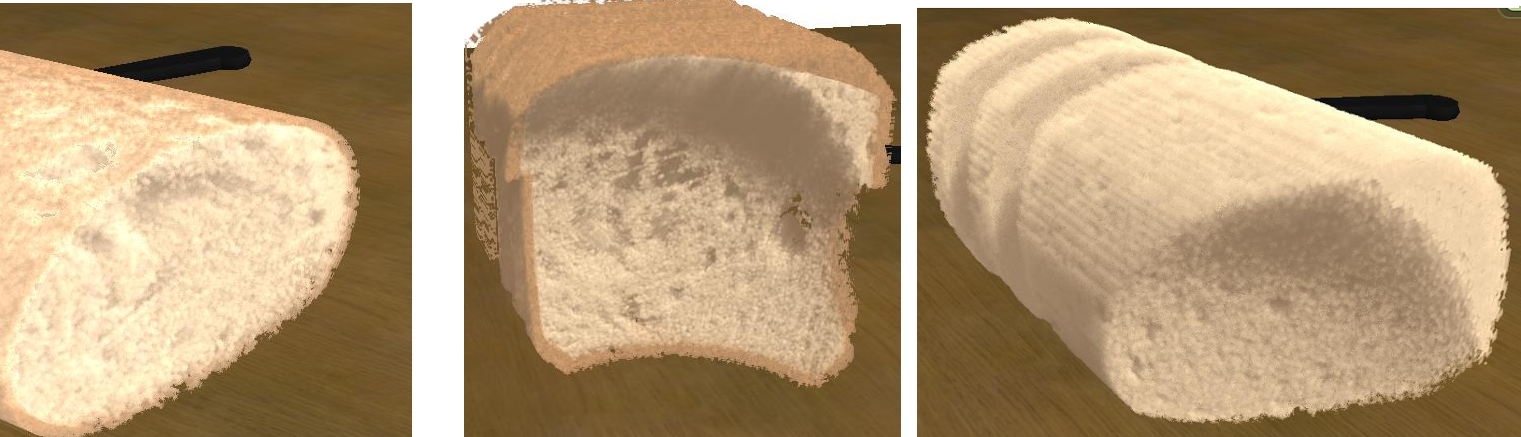
\includegraphics[scale=0.3]{fig5}}
  \caption{Imágenes de diferentes tipos de pan renderizados en tiempo
    real. La imagen de la derecha muestra un pan sin corteza}
  \label{fg:fig5}
\end{figure*}

Es posible obtener otros materiales (ver Fig.~\ref{fg:fig6}). Estos son
el resultado de la variación de parámetros técnicos y artísticos del
modelo. En las imágenes de prueba pueden distinguirse un budín (izquierda), un
pedazo de torta (medio) y una esponja (derecha). En el caso de la esponja
se modificaron los parámetros que definen la función de
densidad. Cuando no hay levadura en el proceso de creación puede
utilizarse una textura volumétrica cuyos valores provienen de una
función aleatoria. La retroiluminación es también aproximada con
este modelo (ver Fig.\ref{fg:fig7}). En esa imagen puede apreciarse
una esponja retroiluminada junto con la propagación de luz a
través del volumen que representa.

\begin{figure*}[htb!]
  \centerline{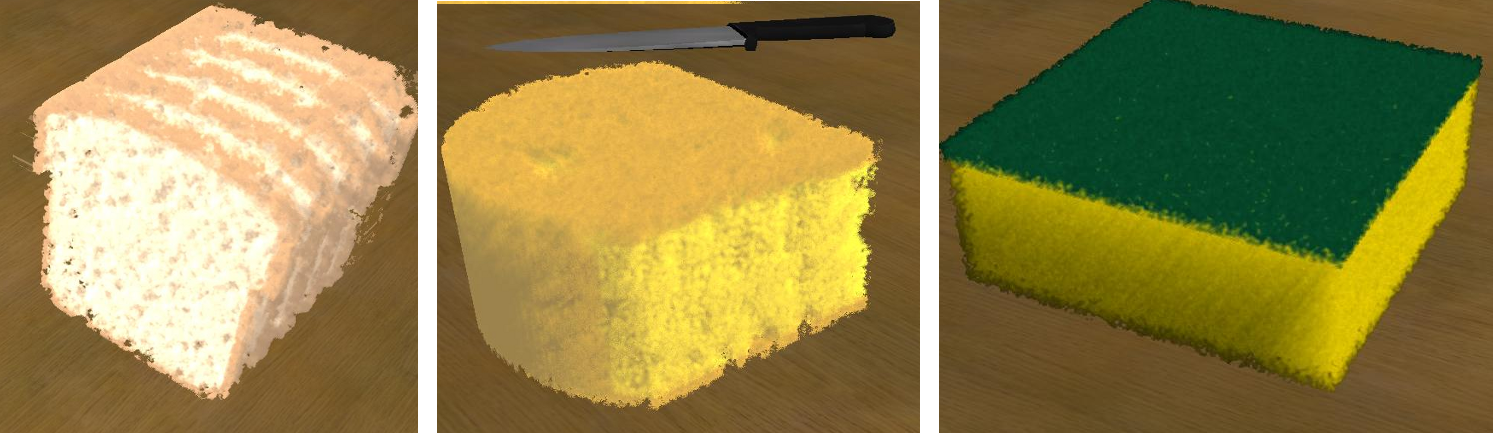
\includegraphics[scale=0.3]{fig6}}
  \caption{Distintos materiales renderizados en tiempo real variando parámetros. Izquierda.: budín, centro: torta, derecha.: esponja. }
  \label{fg:fig6}
\end{figure*}



\begin{figure*}[htb!]
  \centerline{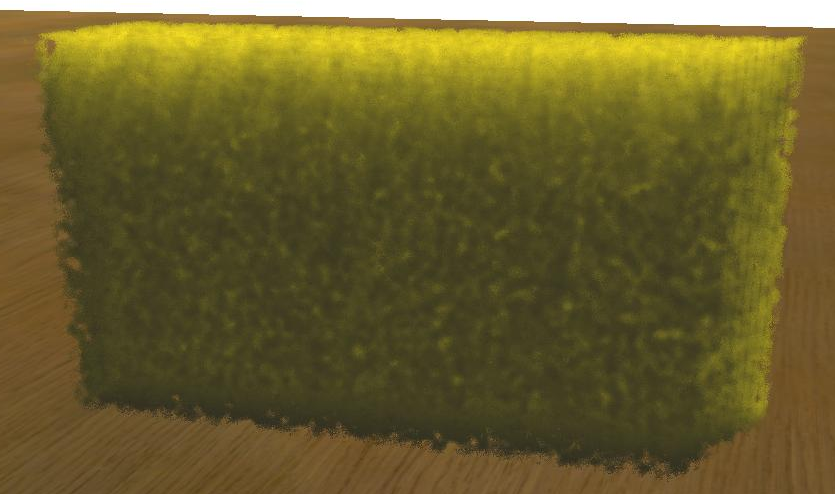
\includegraphics[scale=0.25]{fig7}}
  \caption{Esponja retroiluminada.}
  \label{fg:fig7}
\end{figure*}


\subsection{Tiempos de cómputo}

La mayoría de las imágenes se obtuvieron con tasas de refresco de
tiempo real (más de 30 FPS), como muestra la tabla~\ref{tab:n1}. La
eficiencia del proceso se resiente cuando la transmitancia es muy
baja (el material es casi transparente), dado que se evaluarán más
puntos en los rayos a recorrer antes de llegar al límite de
transmitancia. Otro parámetro importante es la distancia entre puntos
a evaluar. Experimentalmente se encontró que para todos los casos
evaluar $100$ puntos o más presenta buenos resultados. El proceso escala
automáticamente con el numero de procesadores en una GPU, por lo cual
la tasa de refresco obtenida será mayor en GPUs más rápidas y de más
procesadores.

\begin{table}[htb]
\centering
\begin{tabular}{|c|c|c|c|c|c|c|}
\hline &  Pan 1 & Pan 2 & Pan 3 & Budín & Torta & Esponja \\
\hline
\hline
 FPS promedio  & 32.2 &  75.5 &  45.2 & 28.5 &  54.2 & 29.7\\
\hline
 Puntos de evaluación &  140 &  140 &  140 & 256 &  140 & 256 \\
\hline
 Transmitancia &  15 &  15 &  15 & 15 &  15 & 2.25 \\
\hline
\end{tabular}
\caption{Tiempos de cómputo y parámetros de las imágenes de prueba.}
%% \caption{Computing times and key parameters for the images obtained. }
\label{tab:n1}
\end{table}

\subsection{Discusi\'on}

Según el conocimiento de los autores, éste es el primer intento de llevar a cabo una renderización en tiempo real de pan de manera convincente sin el uso de procesos
intermedios complicados (captura de imágenes, generación de mallas,
post-procesamiento). Existen buenos resultados de renderizado de pan
obtenidos con otros métodos \citep{Cho2007}, pero es difícil
comparar ese trabajo con el presentado en este artículo debido a que
ni los detalles de la técnica utilizada ni los tiempos de cálculo han
sido publicados.

Dentro del volumen a renderizar se pueden definir regiones
con diferentes propiedades. Esta idea permite generar
imágenes con miga y corteza con diferentes parámetros.

La integración de la técnica descrita con motores gráficos es
simple. La información de profundidad de los fragmentos puede obtenerse de manera sencilla y por lo tanto pueden utilizarse técnicas
populares de sombras, tales como mapas de sombras.

Los tiempos de cómputo muestran una alta eficiencia del proceso, lo
cual depende en gran medida del número de puntos de evaluación usados
y la transmitancia del material. Sin embargo, tiempos de cómputo
consistentes con aplicaciones de tiempo real pueden alcanzarse en
todos los casos menos en los cuales el volumen ocupa la mayor parte de
la imagen a generar, dado que la técnica se calcula casi enteramente
en los shader de fragmentos. 

Los resultados obtenidos pueden extenderse de diferentes formas, las
cuales se mencionan en la siguiente sección.

%\section{CONCLUSIONS AND FUTURE WORK}


%\subsection{Main headings}

%The main headings should be written left aligned, in 12pt, boldface
%and all capital Times Roman letters. There should be a 12pt space
%before, and 6pt after the main headings.

%\subsection{Secondary headings}

%The secondary headings should be written left aligned, in 12pt,
%boldface Times Roman, with an initial capital for first word only. There
%should be a 12pt space before, and 6pt after the secondary headings.

%\section{TEXT}

%The normal text should be written single-spaced, justified, using 12pt
%Times Roman in one column. The first line of each paragraph must be
%indented 0.5cm. There is not inter-paragraph spacing.

%\section{PAGE NUMBERS}

%The authors {\bf must not number} the pages of the article. Numbers will
%be added by the editor/publisher. 

%\section{FIGURES}

%All figures should be numbered consecutively and captioned. The
%caption should be written centered, in 10pt Times Roman, upper and lower
%case letters.

%\begin{figure*}[htb]
%\centerline{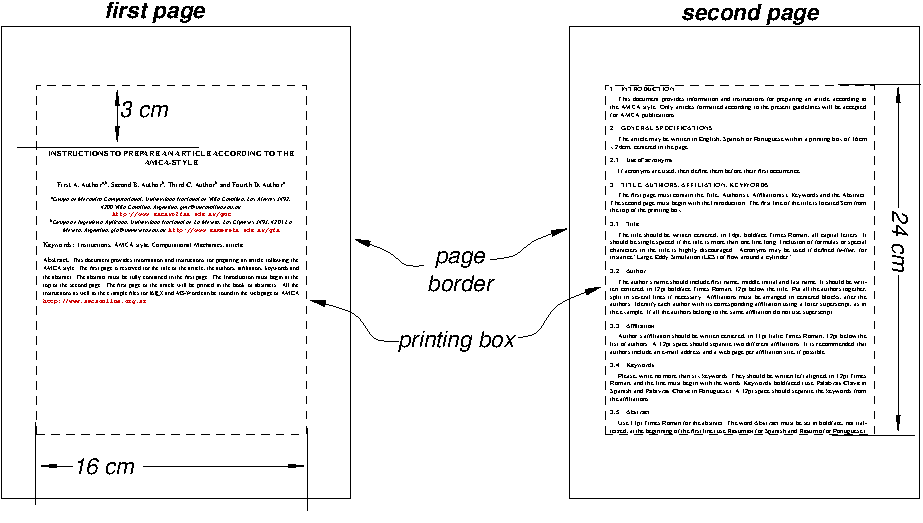
\includegraphics{firstpage}}
%\caption{Page layout}
%\label{fg:figure}
%\end{figure*}

%A 6pt space should separate the figure from the caption, and a
%12pt space should separate the upper part of the figure and the
%bottom of the caption from the surrounding text (see
%Fig.~\ref{fg:figure}).

%Figures should be referenced in the text. Color figures are welcomed.

%\section{EQUATIONS}

%A displayed equation is numbered, using Arabic numbers in parentheses.
%It should be  centered, leaving a 6pt space above and below to separate it from
%the surrounding text.

%The following example is a simple single line
%equation
%
%\begin{equation}
%Ax = b.
%\end{equation}

%The next example is a multi-line equation
%
%\begin{equation} \label{eq:simple}  
%\begin{aligned}
%Ax& = b,\\
%Ax& = c.
%\end{aligned}
%\end{equation}
%
%If possible, internal PDF links must be generated for references to
%equations. The recommended color for links to references in the text
%is blue (e.g., see Eq.~(\ref{eq:simple})).

%\section{TABLES}

%All tables should be numbered consecutively and captioned, the caption
%should be 10pt Times Roman, upper and lower case letters.

%A space of 6pt separates the table from the caption, and 12pt space
%separates the table from the surrounding text. For an example, see
%Table~\ref{tab:n50}. Tables should be referenced in the text.

%\begin{table}[htb]
%\centering
%\begin{tabular}{|c|c|c|c|}
%\hline  & 20x20 mesh & 50x50 mesh & 100x100 mesh\\
%\hline
%\hline
% 0 & 41.00 & 1.00 & 4.92\\
%\hline
% 1 & 40.86 & 1.02 & 4.88 \\
%\hline
%10 & 23.81 & 3.44 & 2.92 \\
%\hline
%50 & 5.62 & 64.20 & 1.08 \\
%\hline
%\end{tabular}
%\caption{Condition number for the Stekhlov operator. }
%\label{tab:n50}
%\end{table}

%\section{FORMAT OF REFERENCES}

%References should be quoted in the text using the \emph{author-style}
%(a.k.a. \emph{Harvard style}). References can be cited in
%\emph{parenthetical} form \citep{zienkiewicz91,idelsohn94,meyer82,meyer82b}, or
%in \emph{textual} form, e.g. see
%\citet{zienkiewicz91,idelsohn94,meyer82,meyer82b}.  References are grouped
%together and sorted alphabetically at the end of the article as shown
%in these instructions. Do not include references that are not cited in
%the article body. 

%If possible, internal PDF links must be generated for citations. The
%recommended color for links to references in the text is blue. The
%preferred color for links to external references, as web pages, 
%is red (e.g. \url{http://www.amcaonline.org.ar}).

\section{CONCLUSIONES}

En este trabajo se aplica el modelo de transmitancia en DVR a un campo escalar 3D el cual representa la estructura de la miga de pan, con el objetivo de obtener im\'agenes foto-real\'isticas del material. Esta estructura se genera utilizando sistemas de part\'iculas, los cuales evolucionan siguiendo sistemas din\'amicos de una manera probabil\'istica. La simulaci\'on se resuelve num\'ericamente. Los resultados muestran im\'agenes con gran resemblanza a im\'agenes del material en tiempo real. Los m\'etodos propuestos pueden aplicarse en distintas \'areas, como juegos serios \citep{Susi2007} y rendering foto-real\'istico. El m\'etodo de rendering no presenta las desventajas de otros m\'etodos del estado del arte.

La principal desventaja del m\'etodo (la cual est\'a presente tambi\'en en los dem\'as m\'etodos del estado del arte) es la resoluci\'on, ya que las placas gr\'aficas tienen un l\'imite en las dimensiones de texturas que soportan. Para resolver este problema, se propone como trabajo futuro setear diferentes texturas volum\'etricas dependiendo de la distancia de la c\'amara al volumen.

Otras posibles continuaciones a este trabajo incluyen mejorar el algoritmo de rendering, buscando tomar en cuenta iluminaci\'on indirecta y difusión de la luz dentro del material. Adem\'as, se tratar\'an ecuaciones diferenciales m\'as generales, para hacer posible una aplicaci\'on directa del modelo matem\'atico del proceso de cocci\'on. Se investigar\'an otros materiales como quesos. Otra idea interesante ser\'ia definir primitivas de miga y corteza permitiendo un modelado art\'istico de estas caracter\'isticas. 

%Template files in TeX, \LaTeX{} and MS-Word may be found at the
%AMCA web site: \url{http://www.amcaonline.org.ar}. 
%Remember: {\bf Do not number the pages.}
%
\bibliography{eniefbib}
\end{document}
% $Id: amcapaper.tex,v 1.23 2006/08/14 16:58:45 mstorti Exp $
